\documentclass[]{article}

% math packages
\usepackage{amsmath}
\usepackage{amsthm}
\usepackage{bm}

% for coloring in a table
%\usepackage[table,xcdraw]{xcolor}

% including graphics
\usepackage{graphicx}
\graphicspath{ {./images/} }

% drawing graphs
\usepackage{tikz-cd}
\usepackage{tikz}
\usetikzlibrary{shapes.geometric, arrows}
\tikzstyle{startstop} = [rectangle, rounded corners, minimum width=3cm, minimum height=1cm,text centered, draw=black, fill=red!10]
\tikzstyle{arrow} = [thick,->,>=stealth]

% hyperlinks
\usepackage{hyperref}

% some useful shortcuts
\DeclareMathOperator*{\argmax}{argmax}
\newcommand{\indep}{\perp\!\!\!\!\perp}
\newcommand{\blambda}{{\bm{\lambda}}}
\newcommand{\btheta}{{\bm{\theta}}}
\newcommand{\bpsi}{{\bm{\psi}}}

\newcommand{\by}{\mathbf{y}}

\usepackage{setspace}
\doublespacing

\usepackage{natbib}
\bibliographystyle{rusnat}

% Editing macros
\usepackage{color}
\newcommand\cmnt[2]{\qquad{{\color{red} \em #1---#2} \qquad}}
\newcommand\cmntM[1]{\cmnt{#1}{Miratrix}}
\newcommand\cmntC[1]{\cmnt{#1}{Che}}
\newcommand\awk{{{\color{red} {$\leftarrow$ Awkward phrasing}}\qquad}}
\newcommand\cmntMp[1]{{\color{red} $\leftarrow$ {\em #1 -Miratrix} \qquad}}



%opening
\title{Power analyses for individual site impacts in multisite trials}
\author{Jonathan Che \& Luke Miratrix}

\begin{document}

\maketitle


\section{Background}

Power analyses for multisite trials generally ensure that a given design will achieve desired levels of power for the overall average treatment effect across all sites. [TODO: add references for prior power analysis stuff for multisite trials, like Kristen’s power formula work, formulas for detecting cross-site impact heterogeneity, etc?] 

In many applications, however, site stakeholders may be interested in estimating treatment effects at the individual sites as well. 
Analysts typically use multilevel models (MLMs) to generate partially pooled estimates of these site-level treatment effects. 
For each site, these models ``borrow strength'' from the other sites, resulting in site-level estimates that are shrunken toward the overall average estimated treatment effect.

The construction of confidence intervals around these shrunken estimates requires some nuance. 
There is an extensive literature concerning the construction of appropriate credible intervals for individual site effects under shrinkage \citep{casella2012shrinkage}.
These credible intervals, however, only satisfy so-called Empirical Bayes (EB) coverage \citep{morris1983parametric}, which means that they only provide guarantees for \textit{average} coverage across sites rather than coverage for any particular site. 
These guarantees may not be sufficient for stakeholders in multisite trials specifically interested in knowing whether an experimental treatment had a positive effect at their site. 
Overall, the question of inference for individual site effects in multilevel models remains fairly open \citep{armstrong2020robust}, with limited guidance about best practices.

In this paper, we conduct power analyses for detecting hypothesized effects for individual sites in multisite trials. 
Similar power analyses have previously been conducted for the overall average treatment effect and cross-site variation in multisite trials (e.g., \citet{raudenbush2000statistical}), but not for individual site-effect estimates, to the best of our knowledge.


\section{Objective}

This paper serves as a guide for practitioners interested in powering their multisite trial analyses to detect individual site-level effects. 
To this end, we conduct power analyses for a suite of popular multilevel modeling methods and provide practical advice for researchers.


\section{Research Design}

We conduct a large-scale simulation study to explore power for individual site-level effects. 
We repeatedly simulate data under a standard normal hierarchical model
% for individuals $i$ in sites $j$ of: 
% \begin{align*}
% 	Y_{ij} &= \alpha_j + \tau_j Z_{ij} + \epsilon_{ij} \\
% 	\alpha_j &= \alpha + u_{0j} \\
% 	\tau_j &= \tau + u_{1j} \\
% 	\begin{pmatrix}
% 		u_{0j} \\ u_{1j}
% 	\end{pmatrix} &\sim N\left(
% 	\begin{pmatrix}
% 		0 \\ 0
% 	\end{pmatrix}, 
% 	\begin{bmatrix}
% 		\sigma^2_\alpha & \rho_{01} \\  & \sigma^2_\tau
% 	\end{bmatrix}\right) \\
% 	\epsilon_{ij} &\sim N(0, \sigma^2_y) ,
% \end{align*}
% for individual outcomes $Y_{ij}$, individual treatment indicators $Z_{ij}$, random site intercepts $\alpha_j$, and random site treatment effects $\tau_j$.
% To simplify things, we will operate in effect-size units, assuming data are rescaled such that $Var(Y_{ij} \mid Z_{ij}=0) = 1$, i.e., that $\sigma^2_y + \sigma^2_\alpha = 1$.
% This also implies that $ICC = \sigma^2_\alpha / (\sigma^2_y + \sigma^2_\alpha) = \sigma^2_\alpha$.
% Finally, we set $\rho_{10} = 0$ so that intercept and treatment random effects are uncorrelated.
where we vary four data-generating parameters: the average size of each site $\bar{n}$, the number of sites $J$, the true overall average treatment effect $\tau$, and the true cross-site variation in site-level effects $\sigma^2_\tau$.
For each simulated dataset, we run four models: a normal Bayesian hierarchical model; a fixed-intercept, random-coefficients (FIRC) model; a random-intercepts, random-coefficients (RIRC) model; and a separate t-test for each site. Finally, we record each model’s estimates of site-level effects and their associated standard errors.

\section{Findings/Results}

Figure \ref{fig:power_plot} visualizes the main power results for one-sided hypothesis tests for the presence of a positive effect at $\alpha=0.1$.
Power is plotted against true $\tau_j$ values for individual sites.
The plots are faceted by $\bar{n}$ and $\sigma_\tau$, $J$ is fixed at $J=100$, and $\tau$ is fixed at $\tau=0.2$.
The horizontal dashed reference lines are at $\alpha = 0.1$ and $0.80$; ideally, the power curve would be less than 0.1 for true ATE values less than or equal to 0, and greater than 0.8 for true ATE values greater than 0.

\begin{figure}[ht]
	\centering
	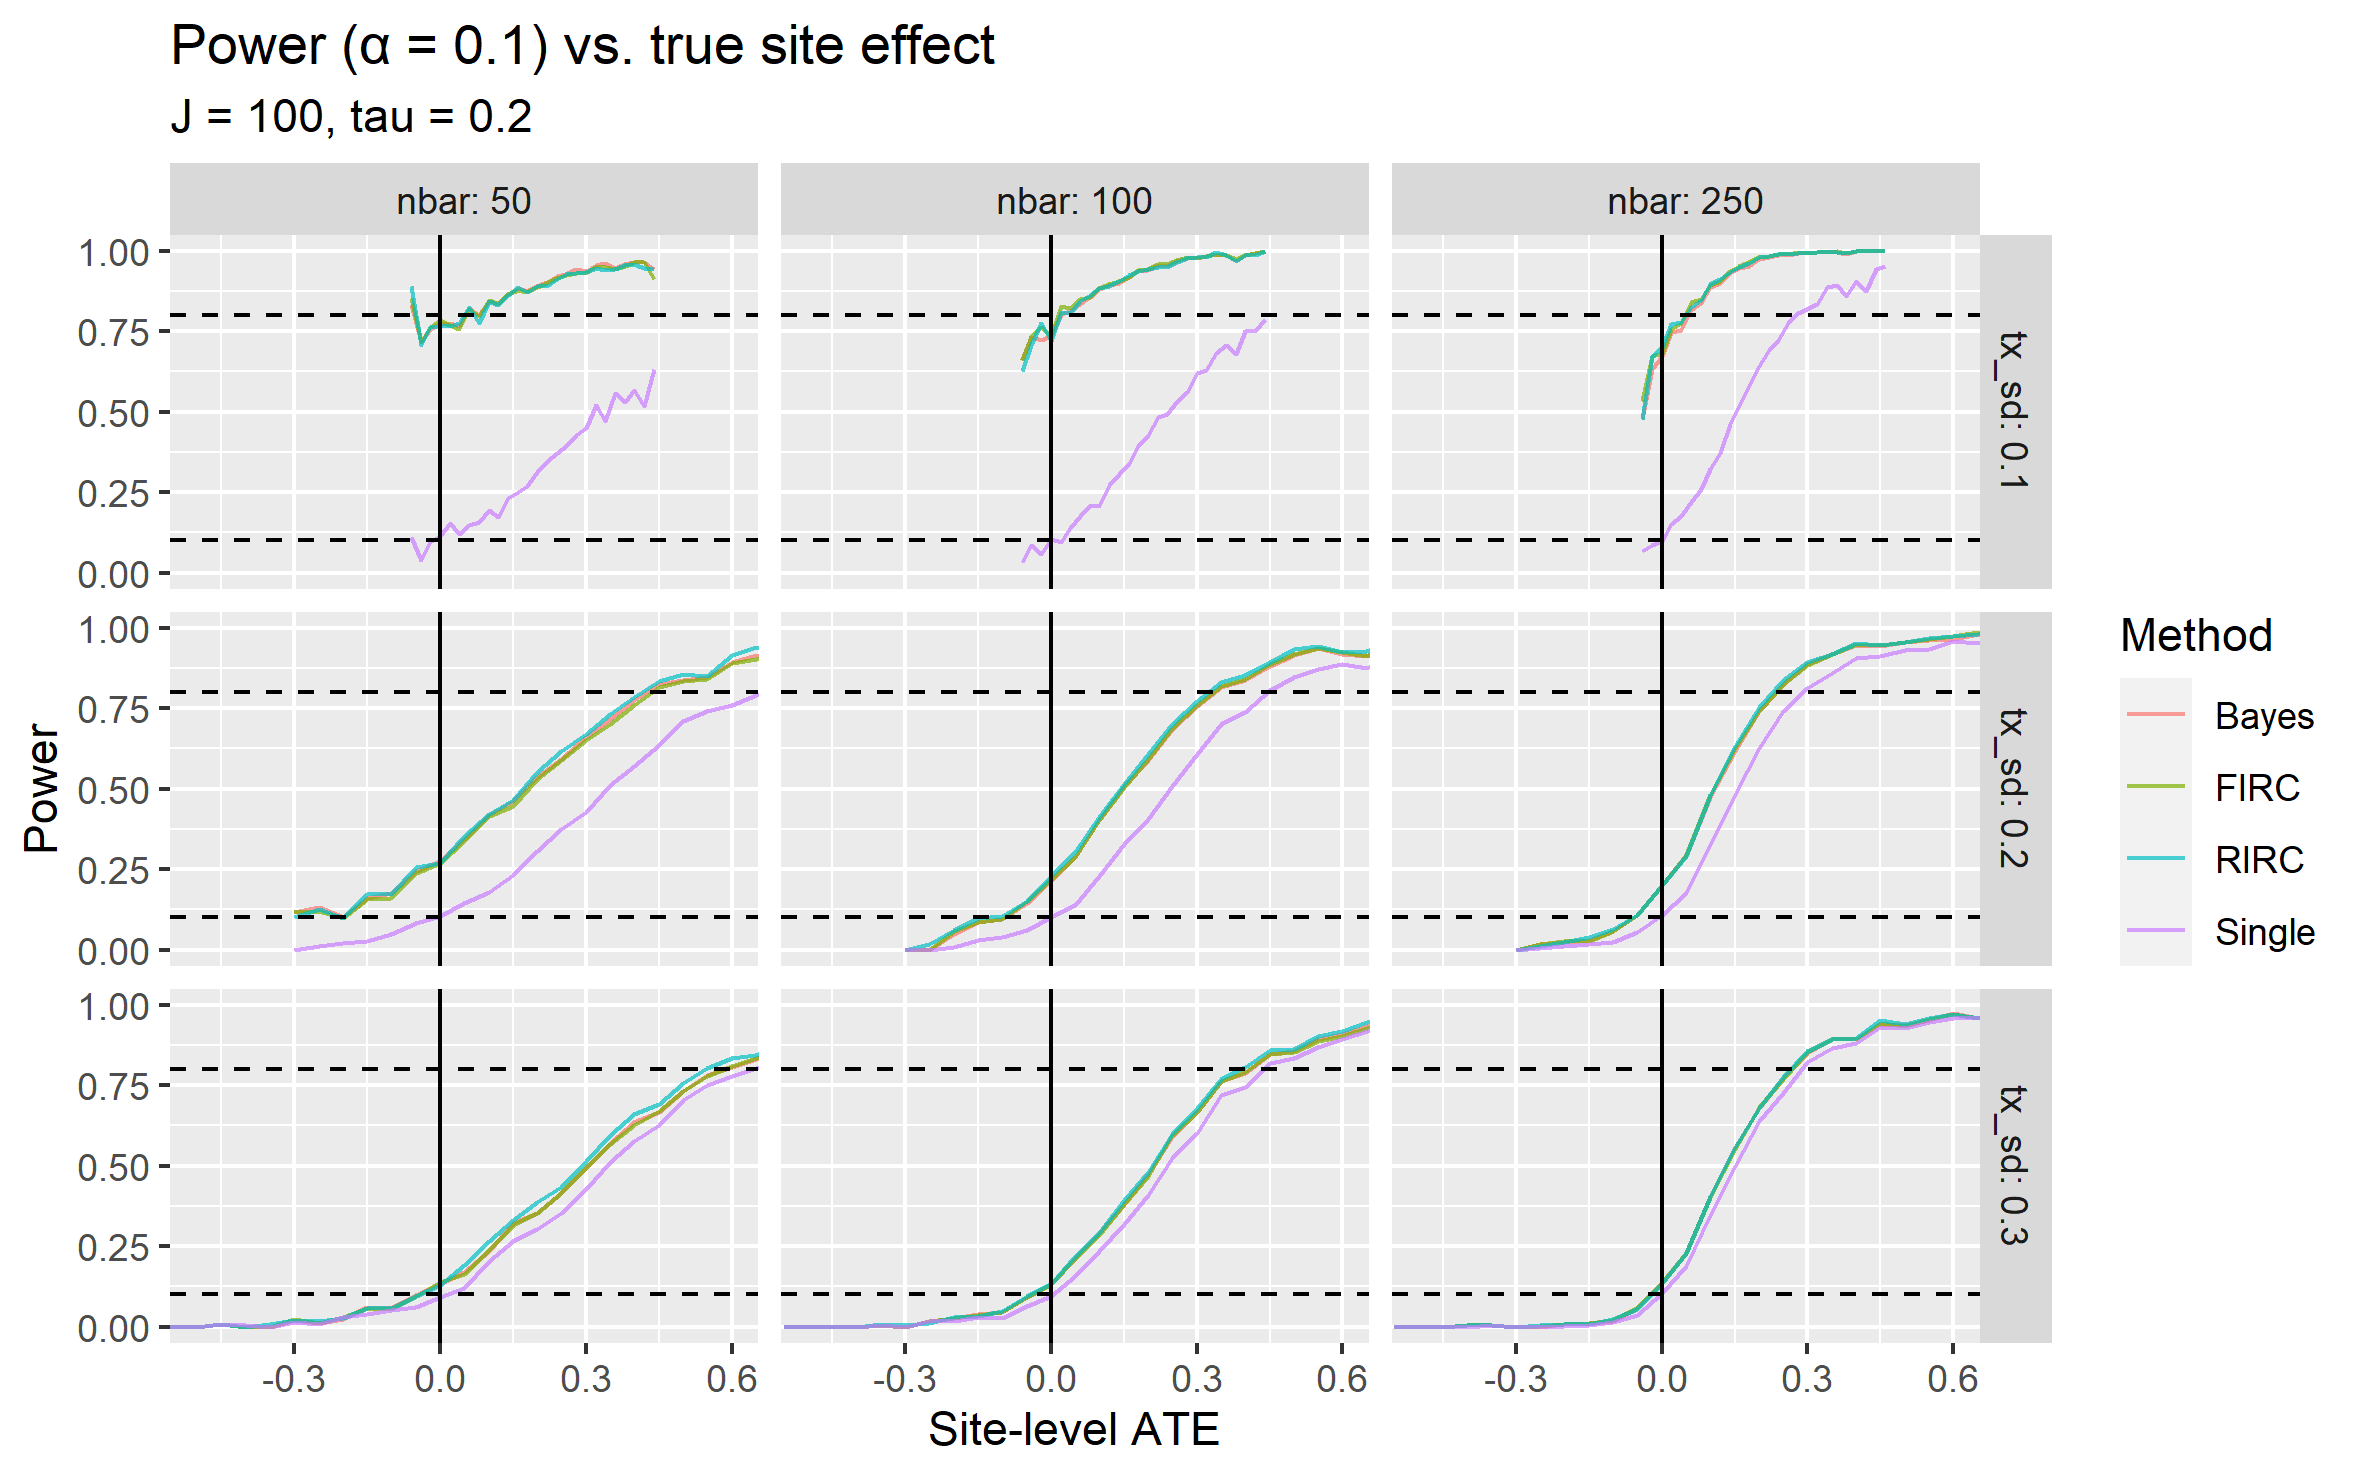
\includegraphics[width=\textwidth]{power_plot_J100}
	\caption{Plot of power (at $\alpha = 0.1$) vs. true site ATE}
	\label{fig:power_plot}
\end{figure}

We see that while using MLMs can improve power relative to using single-site estimates, these improvements often come at the cost of test validity.
This is most extreme in the low-variation setting ($\sigma_\tau = 0.1$), where the false positive rate for sites with negative $\tau_j$ values is nearly 80\%.
In the high-variation, low-information setting ($\bar{n}=50$ and $\sigma_\tau = 0.1$), MLMs provide marginal improvements in power without losing much validity.
Performance between the three MLMs is nearly indistinguishable.

To help illustrate concerns with using MLMs for single-site effect estimates, we can also consider interval coverage properties.
Figure \ref{fig:coverage_plot} plots the Frequentist conditional coverage rate of 90\% two-sided confidence intervals at each true $\tau_j$ value.

\begin{figure}[ht]
	\centering
	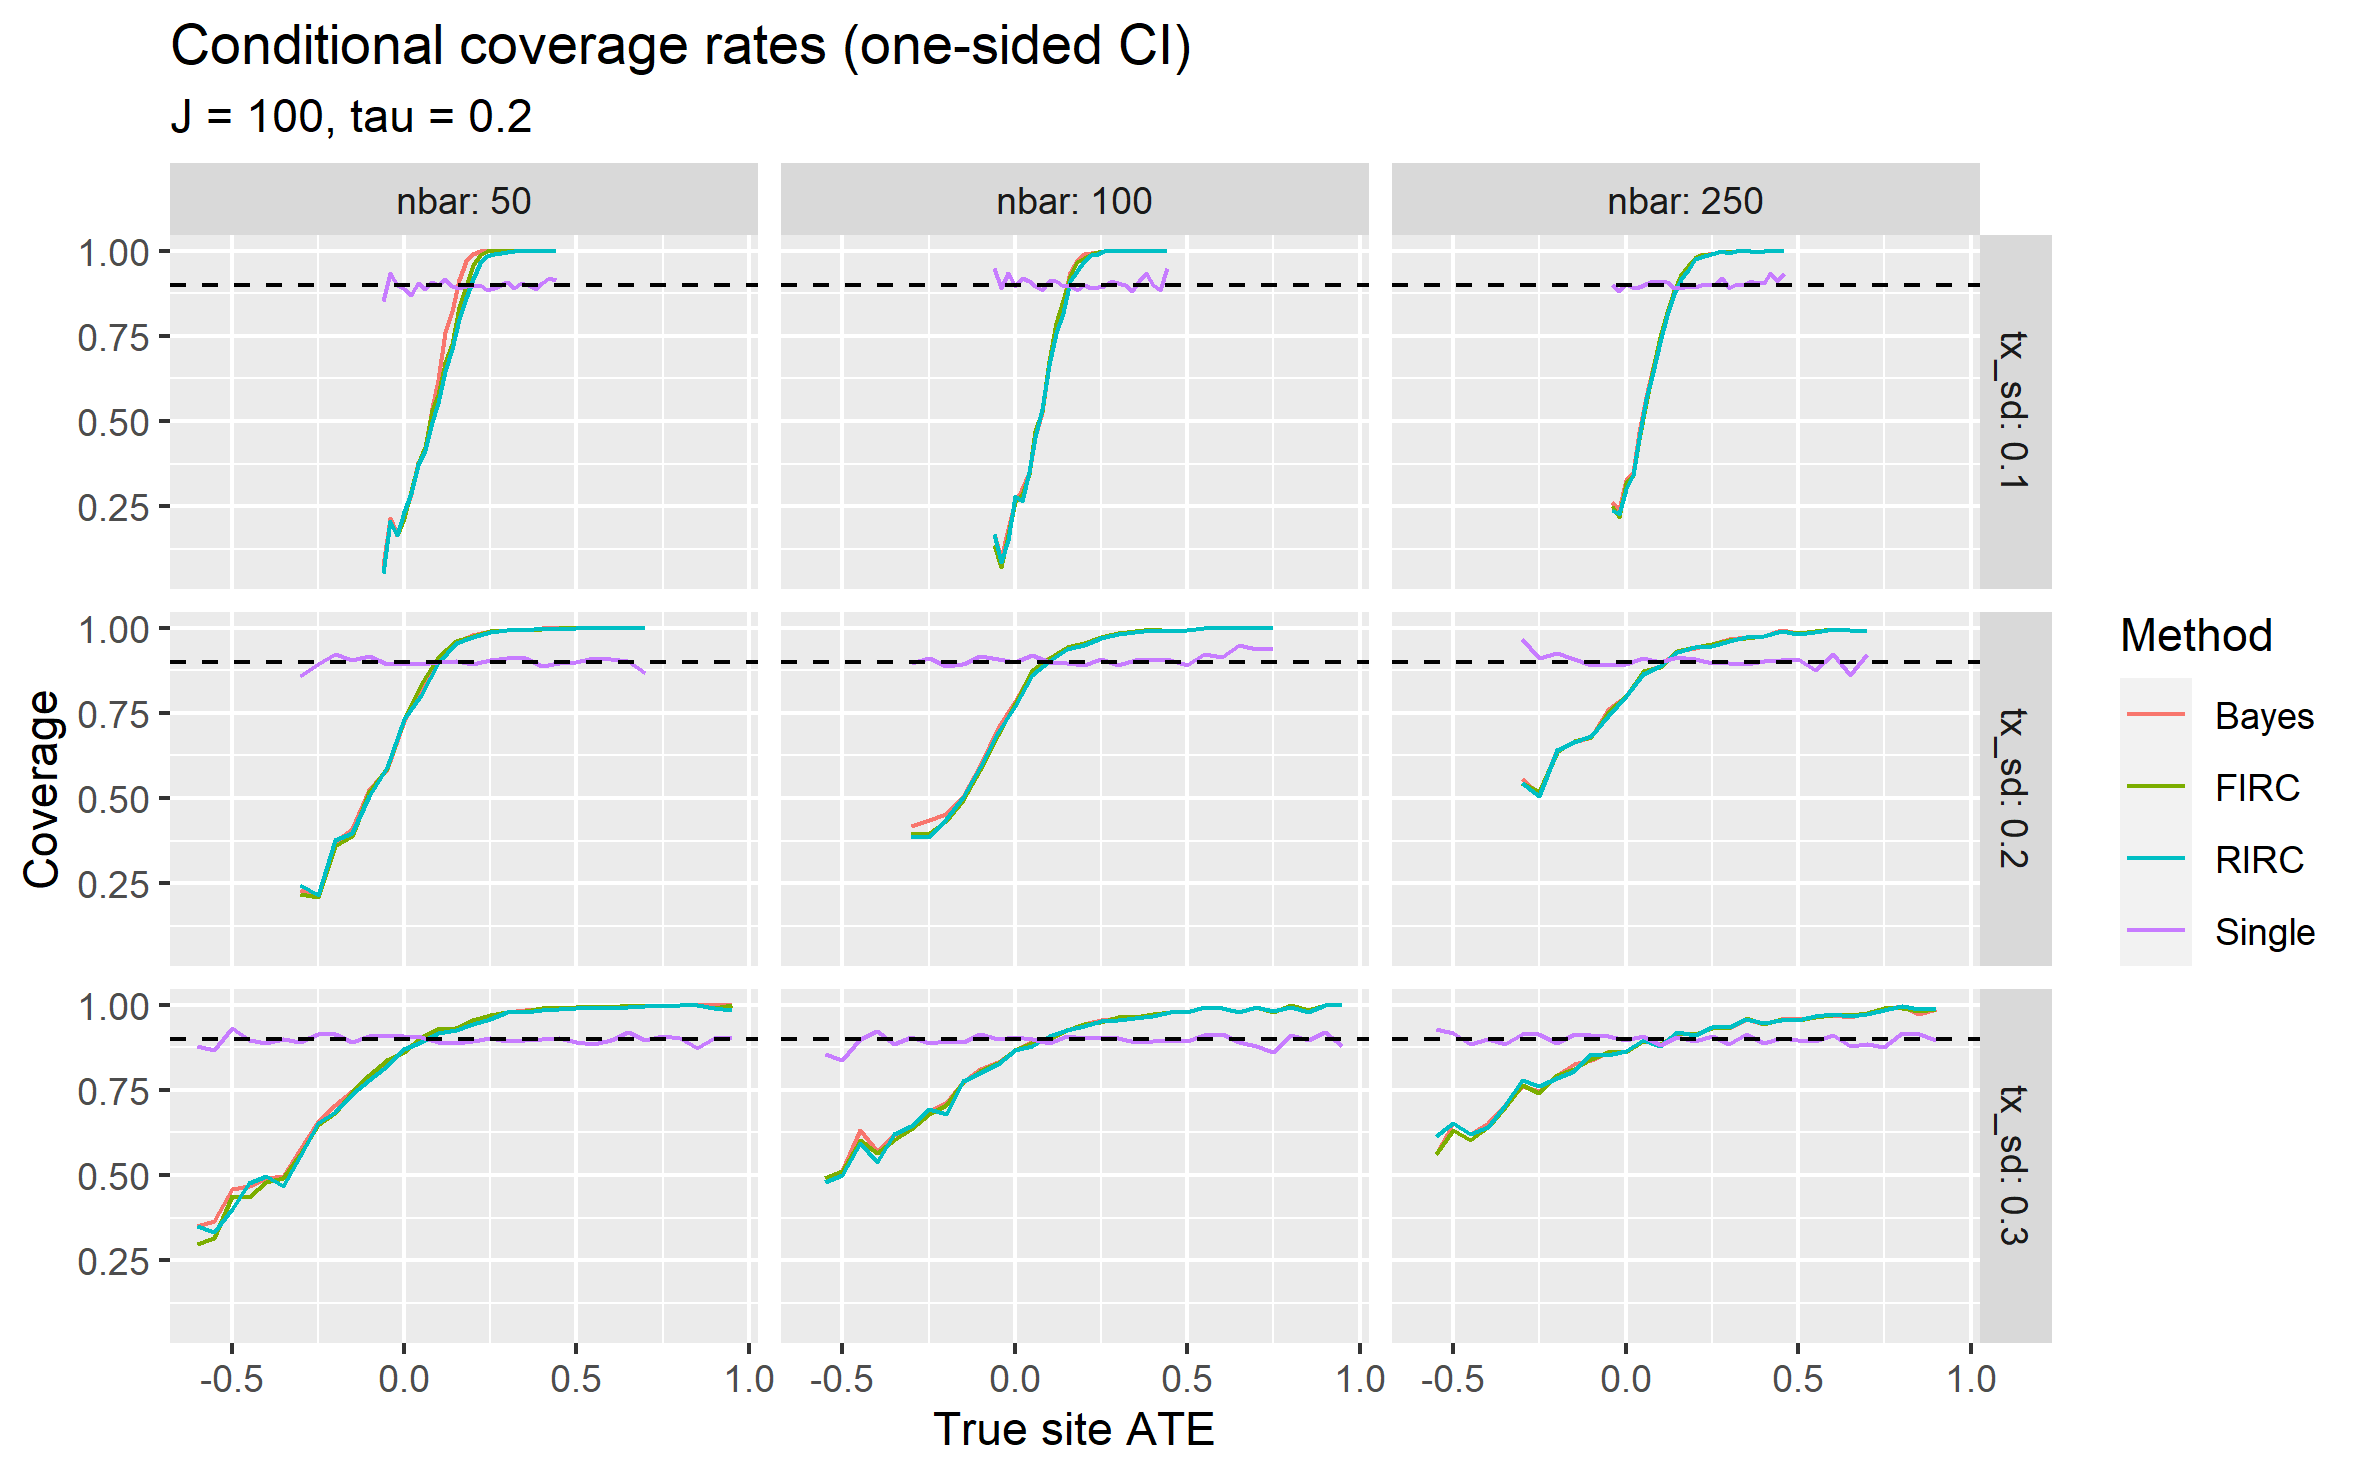
\includegraphics[width=\textwidth]{coverage_plot}
	\caption{Coverage of 90\% confidence intervals for each $\tau_j$ value}
	\label{fig:coverage_plot}
\end{figure}

While the single-site estimates have roughly 90\% coverage regardless of the value of $\tau_j$ as expected, we see curvature in the coverage curves for MLMs; sites with $\tau_j$ values close to $\tau$ are overcovered, and sites with $\tau_j$ values far from $\tau$ are undercovered.
In general, this behavior is expected when examining Frequentist coverage of shrinkage procedures.
Shrinkage causes overcoverage for true parameter values near the center of shrinkage, the true overall average effect of $\tau=0.2$, at the cost of undercoverage for parameter values far from the center of shrinkage.
The curvature in the coverage curve is the most extreme when sites are uninformative (e.g., smaller, so that the model does a significant amount of shrinking), and it becomes less extreme as the sites grow more informative (e.g., larger).

\section{Conclusions}

In many multisite trials, practitioners may be interested in using the estimates produced by MLMs to conduct inference on treatment effects at individual sites.
While MLMs can improve estimation of the overall average treatment effect and cross-site effect heterogeneity, they do not generally improve inferences for individual sites.
In particular, shrinkage can lead to undesirable Frequentist validity and coverage properties, particularly in settings where shrinkage is high.
Practitioners interested in improving power to detect effects at individual sites should aim to make the individual site's estimate more precise, rather than aiming to add other sites to the analysis.

\bibliography{refs.bib}
	
\end{document}